% Provenance (never printed): enseignement scientifique premiere (2019),
% theme "La Terre, un astre singulier: la forme de la Terre" (Eratosthenes,
% meridian measurement by triangulation, the metre); see
% sources/book2/PROVENANCE.md. Every length on the ellipsoid is computed in
% figdata/grade-10/meridian_degree.py (WGS 84, ledger wgs84:ellipsoid).
\chapter{Measuring the Earth}\label{ch:g10:measuring-the-earth}

Stand on a beach and watch a ship sail away towards the open sea. It does not
simply shrink until it is too small to see: first its hull disappears, as if
it were sinking, then the lower part of its superstructure, and the top of
its mast goes last. The sea between you and the ship is not flat; it bulges.
More than twenty-two centuries ago, a scholar of Alexandria turned a similar
observation --- the length of a noon shadow --- into a measurement of the
size of the whole planet. This chapter follows that measurement and those
that came after it: the chains of triangles that surveyors stretched across
countries, the expeditions sent to the Arctic and to the equator to find out
whether the Earth is flattened, the birth of the metre, and the satellites with
which the planet is measured today.

\begin{omfigure}
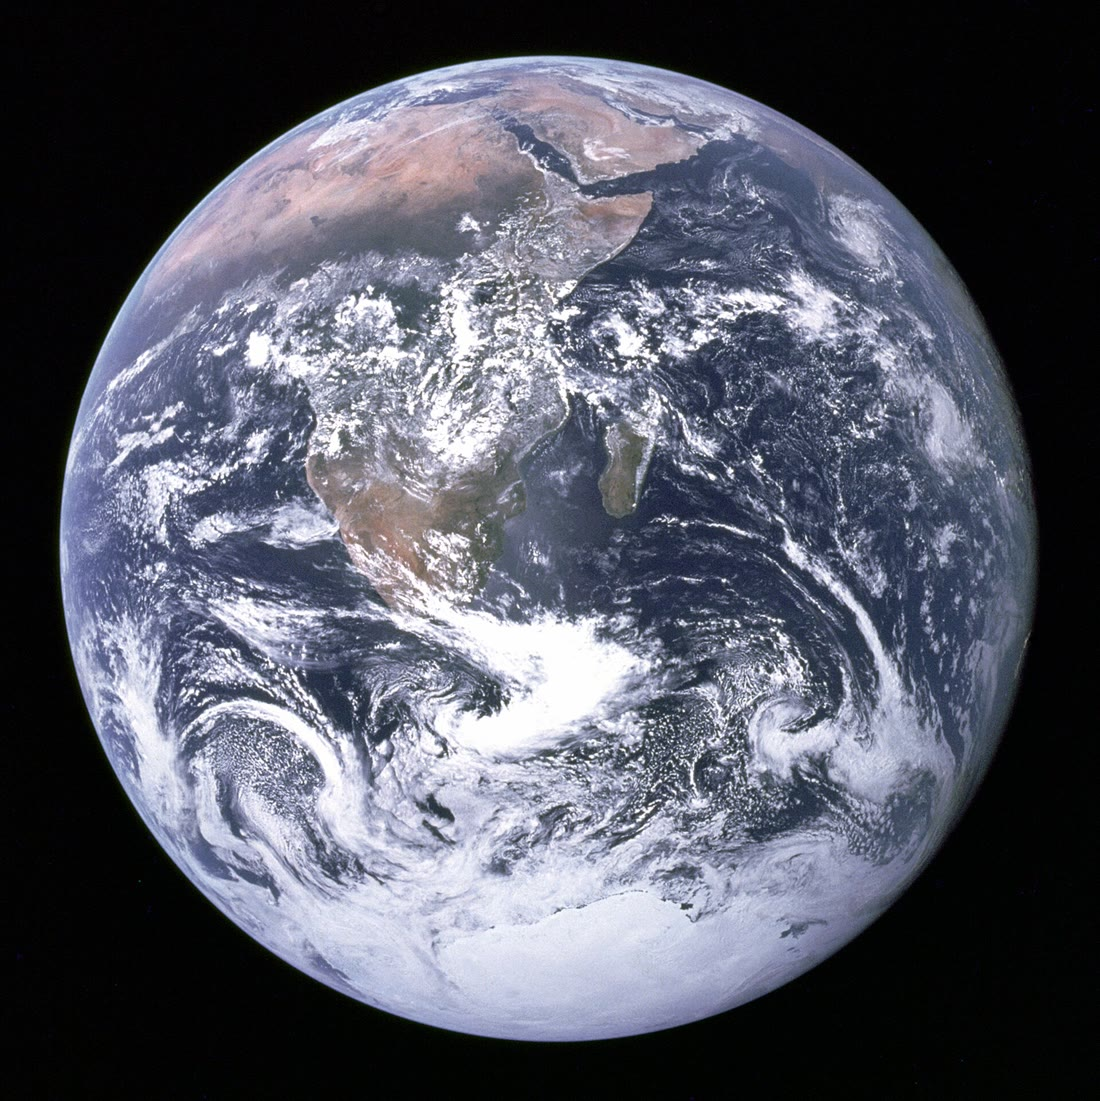
\includegraphics[width=0.5\linewidth]{images/book2/g10-nasa-apollo17-earth.jpg}

{\small The Earth photographed by the crew of Apollo~17 on their way to the
Moon, in December 1972: Africa, Arabia and the ice of Antarctica. Photograph:
NASA (public domain).}
\end{omfigure}

\begin{recall}
A place on the Earth is located by its latitude, its angle north or south of
the equator, and its longitude, its angle east or west of a reference
meridian; meridians join the poles, parallels circle the Earth parallel to
the equator (Book 1). In a uniform medium light travels in straight lines,
and the rays that reach the Earth from the very distant Sun are parallel
(the physics books). In a right triangle, the sine of an acute angle is the
opposite side divided by the hypotenuse, its cosine the adjacent side
divided by the hypotenuse, its tangent the opposite side divided by the
adjacent side (the mathematics books).
\end{recall}

\section{A round Earth}

Long before anyone could look at the Earth from space, several observations
showed that it is round.
\begin{itemize}
  \item \textbf{Ships over the horizon.} A ship sailing away disappears from
        the bottom up, in every direction and on every sea: the surface of
        the sea is curved everywhere.
  \item \textbf{The shadow on the Moon.} During an eclipse of the Moon, the
        Earth's shadow falls on the Moon. Its edge is always an arc of a
        circle, whatever the time of night; only a sphere casts a round
        shadow in every direction.
  \item \textbf{The stars change with latitude.} A traveller going north sees
        the Pole Star climb higher above the horizon, and stars of the
        southern sky disappear below it: the traveller's horizon tilts as
        the traveller moves over a curved surface.
  \item \textbf{Circumnavigation and the view from space.} Ships, then
        aircraft, have travelled around the world in every direction; since
        the 1960s the whole round planet has been photographed.
\end{itemize}

\begin{omfigure}
\begin{tikzpicture}[font=\small, >={Stealth[length=2.2mm]}]
  % sea surface: arc of a circle of radius 8 centred at (0,-8) (curvature exaggerated)
  \fill[omDef!10] plot[domain=-4.6:4.6, samples=60] (\x,{sqrt(64-\x*\x)-8}) -- (4.6,-2.2) -- (-4.6,-2.2) -- cycle;
  \draw[omDef!70!black, thick] plot[domain=-4.6:4.6, samples=60] (\x,{sqrt(64-\x*\x)-8});
  % observer on a small tower at x=-4 (surface y=-1.072), eye at y=-0.235
  \draw[black!70, line width=1pt] (-4,-1.072) -- (-4,-0.235);
  \fill (-4,-0.235) circle (2pt);
  \node[anchor=east, align=right] at (-4.1,-0.2) {observer's\\eye};
  % line of sight tangent at x=-0.5 (y=-0.0156, slope 0.0626)
  \draw[omThm!80!black, thick] (-4,-0.235) -- (4.4,0.290);
  \node[omThm!80!black, anchor=south, rotate=3.6] at (1.3,0.1) {line of sight};
  \fill[omThm!80!black] (-0.5,-0.0156) circle (1.4pt);
  % ship at x=3 (surface y=-0.584), tilted 22 degrees with the local vertical
  \begin{scope}[shift={(3,-0.584)}, rotate=-22]
    \fill[black!12] (-0.6,0) -- (0.6,0) -- (0.75,0.32) -- (-0.75,0.32) -- cycle;
    \draw[black!45, densely dashed] (-0.6,0) -- (0.6,0) -- (0.75,0.32) -- (-0.75,0.32) -- cycle;
    \draw[black!45, densely dashed] (0,0.32) -- (0,0.95);
    \draw[black!80, line width=1pt] (0,0.95) -- (0,1.55);
    \fill[black!80] (0,1.55) -- (0.32,1.25) -- (0,1.25) -- cycle;
  \end{scope}
  \node[anchor=north, align=center, font=\footnotesize] at (2.9,-1.25) {hull and lower mast\\hidden by the bulge};
  \node[anchor=north, font=\footnotesize] at (-0.5,-0.1) {horizon};
\end{tikzpicture}

{\small Why a ship disappears from the bottom up: the observer sees only what
lies above the line of sight that grazes the sea at the horizon. The
curvature is greatly exaggerated.}
\end{omfigure}

\section{Eratosthenes measures the Earth}

Eratosthenes of Cyrene (276--194 BC) was the librarian of Alexandria. He had
heard that at Syene, the present Aswan, far up the Nile, the Sun lit the
whole bottom of a well at noon on the day of the summer solstice: it was
then exactly overhead. At Alexandria, at the same moment, a vertical stick
cast a short shadow: the Sun's rays made an angle of about
\qty{7.2}{\degree} with the vertical, one fiftieth of a full circle.
% ledger: erat:method, erat:stadion

\begin{omfigure}
\begin{tikzpicture}[font=\small, >={Stealth[length=2.2mm]}]
  \def\R{2.4}
  \fill[omDef!8] (0,0) circle (\R);
  \draw[omDef!70!black, thick] (0,0) circle (\R);
  \coordinate (O) at (0,0);
  \coordinate (S) at (\R,0);
  \coordinate (A) at ({\R*cos(25)},{\R*sin(25)});
  \coordinate (T) at ({(\R+0.75)*cos(25)},{(\R+0.75)*sin(25)});
  \coordinate (T2) at ({(\R+1.75)*cos(25)},{(\R+1.75)*sin(25)});
  % radii
  \draw[black!70] (O) -- (S);
  \draw[black!70] (O) -- (A);
  \draw[black!40, densely dashed] (A) -- (T2);
  \fill (O) circle (1.5pt) node[below left] {centre};
  % stick at Alexandria, along the radius
  \draw[line width=1.6pt, black!85] (A) -- ($(A)!0.6!(T)$);
  % well at Syene
  \draw[black!80, thick] ({\R-0.38},-0.12) -- (\R,-0.12) ($(S)+(0,0.12)$) -- ({\R-0.38},0.12);
  % parallel sun rays coming from the right
  \foreach \y in {-1.6,-0.8,0.8,1.6} \draw[->, omThm!70, thick] (6.6,\y) -- (4.4,\y);
  \draw[->, omThm!85!black, thick] (6.6,0) -- (\R+0.05,0);
  \draw[->, omThm!85!black, thick] (6.6,{(\R+0.45)*sin(25)}) -- ({(\R+0.45)*cos(25)+0.03},{(\R+0.45)*sin(25)});
  \node[omThm!85!black, align=center, anchor=west] at (4.6,2.35) {sunlight:\\parallel rays};
  % angles
  \draw[omExo!80!black, thick] (0.75,0) arc (0:25:0.75);
  \node[omExo!80!black] at (1.05,0.22) {$\alpha$};
  \coordinate (Q) at ($(A)!0.6!(T)$);
  \draw[omExo!80!black, thick] ($(Q)+(0.8,0)$) arc (0:25:0.8);
  \node[omExo!80!black] at ($(Q)+({1.08*cos(12.5)},{1.08*sin(12.5)})$) {$\alpha$};
  \node[anchor=east] at ($(A)+(-0.12,0.18)$) {Alexandria};
  \node[anchor=north west] at ($(S)+(0.3,-0.12)$) {Syene};
  \node[font=\footnotesize, anchor=north] at ($(O)!0.5!(S)+(0.2,-0.05)$) {};
  \draw[<->, black!60] ({(\R-0.3)*cos(3)},{(\R-0.3)*sin(3)}) arc (3:22:{\R-0.3});
  \node[anchor=east, font=\footnotesize] at ({(\R-0.35)*cos(13)},{(\R-0.35)*sin(13)}) {$d$};
\end{tikzpicture}

{\small Eratosthenes' reasoning. At Syene the Sun is overhead: its rays point
at the centre of the Earth. At Alexandria a vertical stick, which also points
at the centre, makes an angle $\alpha$ with the rays. The angle at the centre
between the two places is the same $\alpha$. The angle is exaggerated: it was
only \qty{7.2}{\degree}.}
\end{omfigure}

\begin{proposition}[Eratosthenes' relation]\label{prop:g10:measuring-the-earth:eratosthenes}
If two places lie on the same meridian, a distance $d$ apart, and the Sun's
rays at noon make angles with the vertical that differ by $\alpha$ (in
degrees), the circumference of the Earth is
\[
  C = \frac{\qty{360}{\degree}}{\alpha}\, d .
\]
\end{proposition}

\begin{proof}
The Sun is so far away that its rays reaching the two places are parallel.
At each place the vertical points towards the centre of the Earth. In the
figure, the ray reaching the stick and the radius through Syene are two
parallel lines, and the radius through Alexandria crosses both: the angle
$\alpha$ between the stick and the ray and the angle at the centre between
the two radii are alternate angles, hence equal. The arc $d$ is the same
fraction of the whole circumference as the angle $\alpha$ is of a full
turn: $d/C = \alpha/\qty{360}{\degree}$.
\end{proof}

\begin{method}[Measuring a circumference from two shadows]\label{met:g10:measuring-the-earth:shadows}
\begin{enumerate}
  \item Choose two places on (nearly) the same meridian and measure the
        north--south distance $d$ between them.
  \item At local noon on the same day, measure at each place the angle
        between a vertical stick and the Sun's rays: $\tan \theta = s/h$,
        where $h$ is the height of the stick and $s$ the length of its
        shadow. Never look at the Sun itself: the angle is read from the
        shadow alone.
  \item Take the difference $\alpha$ of the two angles and apply
        $C = (360/\alpha)\,d$.
\end{enumerate}
\end{method}

\begin{example}[Eratosthenes' numbers]\label{ex:g10:measuring-the-earth:numbers}
% ledger: erat:method, erat:stadion
Eratosthenes took the distance from Alexandria to Syene to be 5000
\emph{stadia}, a Greek unit of length. With $\alpha = 1/50$ of a circle,
\[
  C = 50 \times 5000 = 250\,000 \text{ stadia}.
\]
How long was a stadion? Historians still debate it. With
\qty{157.2}{m}, $C \approx \qty{39300}{km}$; with \qty{166.7}{m},
$C \approx \qty{41700}{km}$. The true meridian circumference is
\qty{40008}{km}: either way, Eratosthenes was within a few per cent.
\end{example}

\begin{remark}[What was assumed]\label{rem:g10:measuring-the-earth:assumptions}
Eratosthenes assumed a spherical Earth, a Sun far enough for its rays to be
parallel, Syene exactly on the tropic (where the Sun can be overhead), and
Syene due south of Alexandria. Each was nearly but not exactly true: Aswan
lies about \qty{3}{\degree} of longitude east of Alexandria. What matters is
the north--south part of the distance, the one along the meridian.
% ledger: geonames:aswan, geonames:alexandria
\end{remark}

\section{Triangulation}

To measure a long distance on the ground with a chain or a rod is slow, and
across rivers, forests and mountains impossible. Angles, on the other hand,
can be measured very precisely with a telescope on a graduated circle,
pointed in turn at two distant signals. From the eighteenth century on,
surveyors used this to measure whole countries.

\begin{definition}[Geodesy]\label{def:g10:measuring-the-earth:geodesy}
\emph{Geodesy}\index{geodesy} is the science that measures the shape and
the size of the Earth and the positions of points on its surface, and
follows how they change with time.
\end{definition}

\begin{definition}[Triangulation]\label{def:g10:measuring-the-earth:triangulation}
\emph{Triangulation}\index{triangulation} locates distant points by a chain
of triangles: one side, the \emph{baseline}, is measured on the ground with
great care; all the angles of the triangles are measured from their
corners; every other side is then computed.
\end{definition}

The computation rests on one relation between the sides and the angles of
any triangle. In a triangle $ABC$, write $a$, $b$, $c$ for the sides
opposite the corners $A$, $B$, $C$, and $A$, $B$, $C$ also for the angles at
these corners.

\begin{proposition}[The sine rule]\label{prop:g10:measuring-the-earth:sine-rule}
In any triangle $ABC$,
\[
  \frac{a}{\sin A} = \frac{b}{\sin B} = \frac{c}{\sin C}.
\]
\end{proposition}

\begin{proof}
Draw the height from $C$, meeting the line $AB$ at $H$ (second panel of the
figure below); write $h = CH$. In the right triangle $AHC$, $\sin A = h/b$,
so $h = b \sin A$. In the right triangle $BHC$, $\sin B = h/a$, so
$h = a \sin B$. Hence $b \sin A = a \sin B$, that is $a/\sin A = b/\sin B$.
(If the angle at $B$ is obtuse, $H$ falls beyond $B$ and the angle of the
right triangle at $B$ is $\qty{180}{\degree} - B$, which has the same sine.)
The same argument with the height from $A$ gives $b/\sin B = c/\sin C$.
\end{proof}

\begin{omfigure}
\begin{tikzpicture}[font=\small, >={Stealth[length=2mm]}]
  \begin{scope}
    \coordinate (A) at (0,0); \coordinate (B) at (2.0,0.25);
    \coordinate (C) at (0.9,1.9); \coordinate (D) at (3.0,2.1);
    \coordinate (E) at (1.9,3.8); \coordinate (F) at (3.9,4.1);
    \coordinate (G) at (2.7,5.6);
    \draw[black!60] (A) -- (C) -- (B) (C) -- (D) -- (B) (C) -- (E) -- (D) -- (F) -- (E) -- (G) -- (F);
    \draw[omThm!85!black, line width=2pt] (A) -- (B);
    \foreach \p in {A,B,C,D,E,F,G} \fill (\p) circle (1.6pt);
    \node[below left] at (A) {$A$}; \node[below right] at (B) {$B$};
    \node[left] at (C) {$C$}; \node[right] at (D) {$D$};
    \node[left] at (E) {$E$}; \node[right] at (F) {$F$}; \node[above] at (G) {$G$};
    \node[omThm!85!black, anchor=north, font=\footnotesize] at (1.25,-0.3) {measured baseline};
    \draw[omExo!80!black] ($(A)!0.28!(B)$) arc[start angle=7, end angle=64.6, radius=0.56];
    \draw[omExo!80!black] ($(B)!0.3!(A)$) arc[start angle=187, end angle=123, radius=0.6];
    \draw[black!50, densely dashed] (-0.5,0) -- (-0.5,5.6);
    \draw[->, black!70] (-0.5,5.0) -- (-0.5,5.8) node[above] {N};
    \node[rotate=90, font=\footnotesize, black!60, anchor=south] at (-0.5,2.6) {meridian};
  \end{scope}
  \begin{scope}[xshift=6.2cm, yshift=0.6cm]
    \coordinate (A) at (0,0); \coordinate (B) at (4,0); \coordinate (C) at (1.4,2.6);
    \coordinate (H) at (1.4,0);
    \draw[thick] (A) -- (B) -- (C) -- cycle;
    \draw[omDef!80!black, densely dashed] (C) -- (H);
    \draw[omDef!80!black] (1.4,0.22) -- (1.62,0.22) -- (1.62,0);
    \node[below left] at (A) {$A$}; \node[below right] at (B) {$B$};
    \node[above] at (C) {$C$}; \node[below] at (H) {$H$};
    \node[omDef!80!black, anchor=west] at (1.4,1.05) {$h$};
    \node[anchor=south east] at (0.7,1.3) {$b$};
    \node[anchor=south west] at (2.75,1.35) {$a$};
    \node[anchor=north] at (2.7,-0.02) {$c$};
    \draw[omExo!80!black] (0.5,0) arc (0:61.7:0.5);
    \draw[omExo!80!black] (3.45,0) arc (180:135:0.55);
  \end{scope}
\end{tikzpicture}

{\small Left: a chain of triangles stretched along a meridian from a
measured baseline $AB$; the arcs mark two of the many angles measured with
the instrument. Right: the height $h$ from $C$, written in two ways, gives
the sine rule.}
\end{omfigure}

\begin{method}[Computing a triangulation chain]\label{met:g10:measuring-the-earth:chain}
\begin{enumerate}
  \item In the first triangle $ABC$, the baseline $c = AB$ and the angles at
        $A$ and $B$ are measured; the third angle is
        $C = \qty{180}{\degree} - A - B$ (and its measurement checks the
        others).
  \item The sine rule gives the two other sides:
        $b = AC = c \sin B / \sin C$ and $a = BC = c \sin A / \sin C$.
  \item A computed side becomes the known side of the next triangle, and so
        on along the chain.
  \item Finally, the north--south part of each side is computed with the
        cosine of its angle to the meridian, and the parts are added.
\end{enumerate}
\end{method}

\begin{example}[One triangle]\label{ex:g10:measuring-the-earth:triangle}
A baseline $AB = \qty{8.000}{km}$ is measured; from $A$ the signal $C$ is
seen at \qty{70}{\degree} from the direction of $B$, from $B$ at
\qty{60}{\degree} from the direction of $A$. Then $C = \qty{50}{\degree}$ and
\[
  AC = \frac{8.000 \times \sin 60^\circ}{\sin 50^\circ} = \frac{8.000 \times 0.8660}{0.7660}
  \approx \qty{9.044}{km}, \qquad
  BC = \frac{8.000 \times \sin 70^\circ}{\sin 50^\circ} \approx \qty{9.814}{km}.
\]
No distance but the baseline was walked.
\end{example}

\begin{example}[The meridian of the metre]\label{ex:g10:measuring-the-earth:meridian}
% ledger: metre:1791, metre:survey, geonames:dunkirk, geonames:barcelona (arc computed in figdata/grade-10/meridian_degree.py)
In March 1791 the metre was defined as one ten-millionth of the distance
from the pole to the equator along a meridian. To find that distance, two
astronomers, Jean-Baptiste Delambre and Pierre Méchain, measured by
\omterm{def:g10:measuring-the-earth:triangulation}{triangulation} the meridian arc from Dunkirk, on the North Sea, to
Barcelona, on the Mediterranean --- almost seven years of work, Delambre in
the northern two thirds, Méchain in the southern third. The two towns differ
by \qty{9.646}{\degree} of latitude; on the modern ellipsoid the arc between
their parallels is \qty{1072.2}{km} long. Knowing the length of an arc and its
difference in latitude gives the length of a degree; the shape of the Earth
then gives the whole quarter meridian. Platinum standards of the new metre
were made in 1799 and kept in the national Archives.
\end{example}

\begin{history}[The repeating circle]
The angles of the meridian of the metre were measured with a \emph{repeating
circle}, an instrument built by Jean-Charles de Borda: two telescopes on a
graduated circle, pointed alternately at two signals many times over, so
that the errors of reading the graduation are divided by the number of
repetitions.
\begin{center}
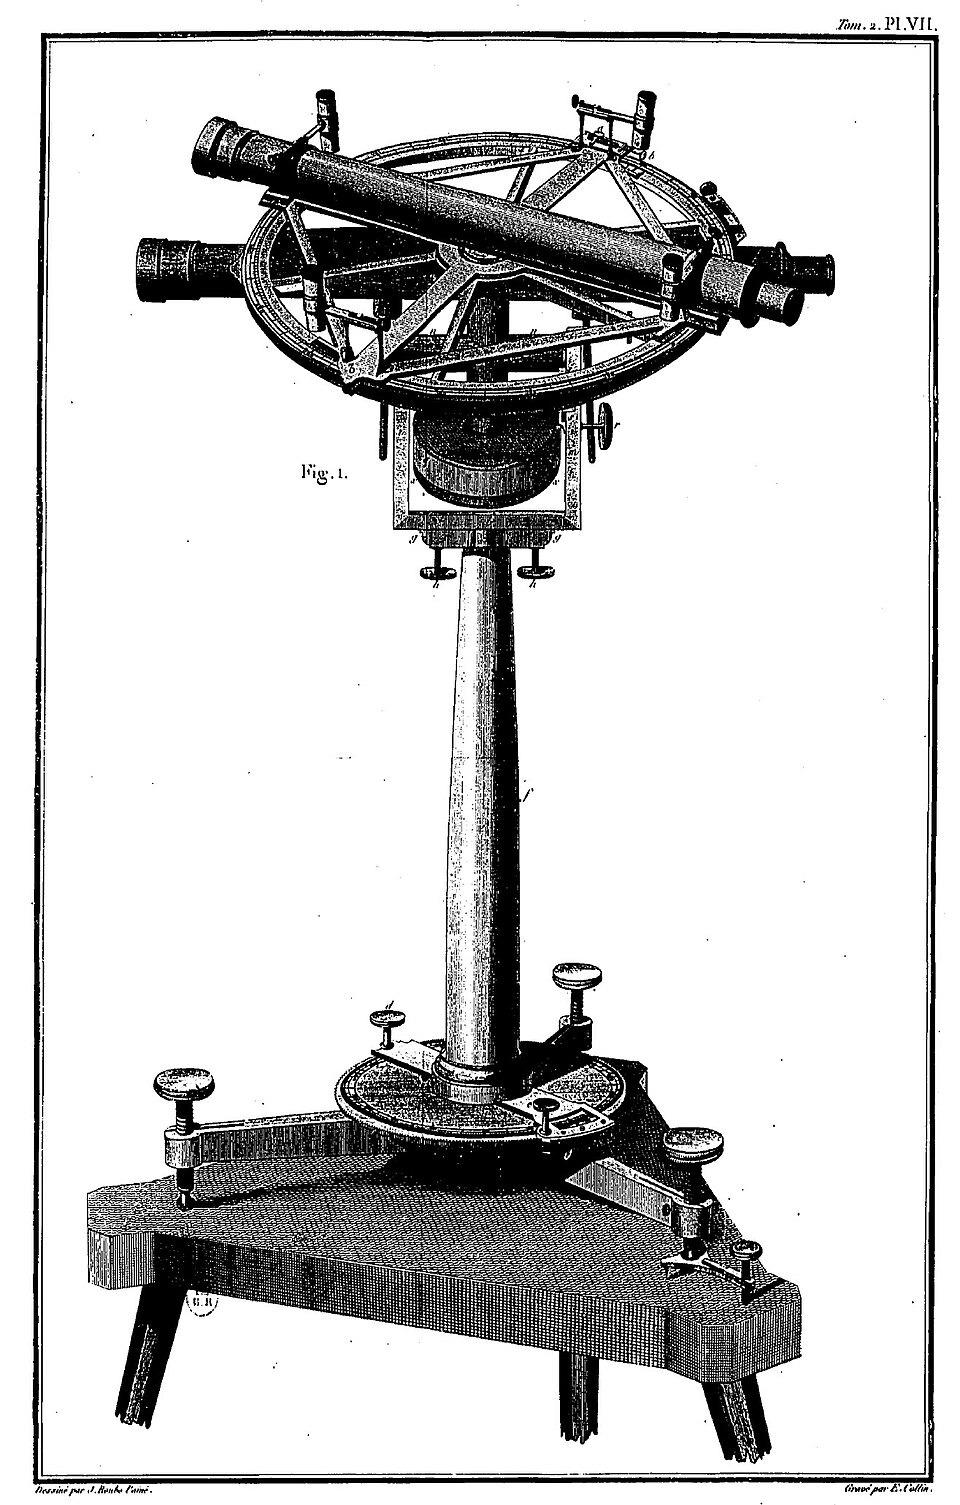
\includegraphics[width=0.3\linewidth]{images/book2/g10-delambre-repeating-circle.jpg}

{\small A repeating circle set up to measure horizontal angles, as engraved
in Delambre's account of the measurement (1807). Public domain (Wikimedia
Commons).}
\end{center}
\end{history}

\section{A flattened Earth}

Around 1687, Isaac Newton argued from his theory of gravitation that a
rotating Earth must be a spheroid flattened at the poles and bulging at the
equator. Measurements of degrees of the meridian made by the astronomers of
the Paris Observatory seemed to say the opposite: an Earth elongated at the
poles. The question was settled by measuring the length of one degree of
latitude as far apart as possible.
% ledger: figure:expeditions

\begin{omfigure}
\begin{tikzpicture}[font=\small, >={Stealth[length=2mm]}]
  \def\a{3.0} \def\b{2.3}
  \draw[black!35, densely dashed] (0,0) circle (\a);
  \fill[omDef!8] (0,0) ellipse ({\a} and {\b});
  \draw[omDef!70!black, thick] (0,0) ellipse ({\a} and {\b});
  \draw[black!50] (-3.4,0) -- (3.7,0);
  \draw[black!50] (0,-2.6) -- (0,3.3);
  \draw[<->, omThm!85!black] (0,-0.3) -- (\a,-0.3);
  \node[omThm!85!black, below] at (1.5,-0.3) {$a$};
  \draw[<->, omThm!85!black] (-0.3,0) -- (-0.3,\b);
  \node[omThm!85!black, left] at (-0.3,1.15) {$b$};
  \node[above right] at (0,\b) {N};
  \node[anchor=south east] at (3.0,-2.5) {};
  \node[anchor=west] at (3.7,0) {equator};
  % normal at t = 45 deg: P = (2.121, 1.626); crosses the equator at (0.874,0), the axis at (0,-1.14)
  \coordinate (P) at (2.121,1.626);
  \draw[omExo!85!black, thick] (P) -- ($(P)!1.35!(0.874,0)$);
  \draw[omExo!85!black, thick, ->] (P) -- ($(P)!-0.45!(0.874,0)$);
  \fill (P) circle (1.6pt);
  \node[anchor=west, align=left, font=\footnotesize] at (2.85,2.35) {local vertical\\(plumb line)};
  \draw[omExo!85!black] (1.45,0) arc (0:52.5:0.58);
  \node[omExo!85!black] at (1.62,0.32) {$\varphi$};
  \fill (0,0) circle (1.3pt);
  \node[anchor=north east, font=\footnotesize] at (0,0) {centre};
  \node[black!50, font=\footnotesize, anchor=south] at (-2.2,2.15) {sphere};
\end{tikzpicture}

{\small A flattened Earth, with the \omterm{def:g10:measuring-the-earth:ellipsoid}{flattening} greatly exaggerated (the true
one is too small to see at this scale). The vertical at a place is
perpendicular to the surface; it does not point exactly at the centre. The
latitude $\varphi$ of the place is the angle between its vertical and the
plane of the equator.}
\end{omfigure}

Latitude is measured from the stars: it is the angle between the local
vertical and the plane of the equator. On a flattened Earth the surface is
less curved near the poles than near the equator. Where the surface is less
curved, one must travel farther along it for the vertical to turn by one
degree: \emph{a degree of latitude is longer near the poles}.

\begin{history}[Lapland and Peru]
% ledger: figure:expeditions, figure:degrees
In 1735 the Paris Academy of Sciences sent an expedition to the equator, in
the Spanish province of Peru (now Ecuador); it worked there for nine years,
until 1744. In 1736--1737 a second expedition, led by Pierre-Louis Moreau de
Maupertuis with the young mathematician Alexis Clairaut, measured a degree
of the meridian in Lapland, near the Arctic Circle. The Lapland degree came
out at 57\,437 \emph{toises} (the old unit of length; about
\qty{111.95}{km}), the Peru degree at only 56\,737 toises: the degree is
longer near the pole, and Newton was right. The two numbers implied a
\omterm{def:g10:measuring-the-earth:ellipsoid}{flattening} of about $1/205$ --- too large, as later surveys showed, but the
question of the sign was settled.
\end{history}

\begin{omfigure}
\begin{tikzpicture}
\begin{axis}[omrecord, width=0.82\linewidth, height=5.4cm, xmin=0, xmax=90,
  ymin=110.45, ymax=111.8, xlabel={latitude (\unit{\degree})},
  ylabel={length of \qty{1}{\degree} of latitude (km)}, xtick={0,15,...,90},
  ytick={110.6,110.8,...,111.8}, yticklabel style={/pgf/number format/fixed, /pgf/number format/fixed zerofill, /pgf/number format/precision=1}]
\addplot[omDef!85!black, line width=1.1pt] table[x=lat_deg, y=deg_km] {figdata/out/grade-10-meridian_degree.dat};
\addplot[only marks, mark=*, mark size=1.8pt, omThm!85!black] coordinates {(0,110.574) (45,111.132) (66,111.507) (90,111.694)};
\node[anchor=south west, font=\footnotesize] at (axis cs:2,110.6) {110.57 km};
\node[anchor=north east, font=\footnotesize] at (axis cs:89,111.56) {111.69 km};
\node[anchor=north west, font=\footnotesize] at (axis cs:46,111.12) {111.13 km};
\node[anchor=south east, font=\footnotesize] at (axis cs:65,111.53) {111.51 km at \ang{66} (Lapland)};
\end{axis}
\end{tikzpicture}

{\small The length of one degree of latitude on the \omterm{def:g10:measuring-the-earth:ellipsoid}{reference ellipsoid} of
\cref{def:g10:measuring-the-earth:ellipsoid}, from the equator to the pole.
Computed from the WGS~84 ellipsoid.}
\end{omfigure}

\begin{definition}[Reference ellipsoid and flattening]\label{def:g10:measuring-the-earth:ellipsoid}
A \emph{reference ellipsoid}\index{reference ellipsoid} is the surface
obtained by rotating an ellipse about its short axis, chosen to fit the
shape of the Earth as closely as possible. Its \emph{equatorial radius} is
$a$, its \emph{polar radius} $b$, and its
\emph{flattening}\index{flattening} is
\[
  f = \frac{a-b}{a}.
\]
\end{definition}

\begin{proposition}[The dimensions of the Earth]\label{prop:g10:measuring-the-earth:dimensions}
% ledger: wgs84:ellipsoid, earth:Req, earth:Rpol, earth:Rmean (lengths computed in figdata/grade-10/meridian_degree.py)
The \omterm{def:g10:measuring-the-earth:ellipsoid}{reference ellipsoid} used by satellite positioning (WGS~84) has
\[
  a = \qty{6378.137}{km}, \qquad b = \qty{6356.752}{km}, \qquad
  f = \frac{1}{298.257}.
\]
The polar radius is \qty{21.4}{km} shorter than the equatorial radius. The
equator is \qty{40075}{km} long and a meridian, from pole to pole and back,
\qty{40008}{km}; the quarter meridian, from the equator to a pole, is
\qty{10001.966}{km}. One degree of latitude is \qty{110.574}{km} long at the
equator and \qty{111.694}{km} at the poles. A degree of longitude is
\qty{111.32}{km} long on the equator and shrinks towards the poles about as
$\cos \varphi$.
\end{proposition}

\begin{example}[A degree of longitude]\label{ex:g10:measuring-the-earth:longitude}
A parallel at latitude $\varphi$ is a circle whose radius is the distance
from the axis, about $R \cos \varphi$. At \qty{60}{\degree} N its
circumference is about half that of the equator, and a degree of longitude
is about $111.32 \times \cos 60^\circ \approx \qty{55.7}{km}$ (the
ellipsoid gives \qty{55.80}{km}).
\end{example}

\begin{remark}[How round is round?]\label{rem:g10:measuring-the-earth:round}
A \omterm{def:g10:measuring-the-earth:ellipsoid}{flattening} of $1/298$ is small. On a globe \qty{30}{cm} across, the polar
diameter would be only \qty{1}{mm} shorter than the equatorial one ---
invisible. The deepest ocean trench, nearly \qty{11}{km} below sea level,
would be a scratch about a quarter of a millimetre deep. For most purposes the Earth is a
sphere of mean radius \qty{6371}{km}; for precise positions, the ellipsoid
is needed.
% ledger: earth:Rmean, usgs:trench-depth
\end{remark}

\section{Geodesy today}

\begin{omfigure}
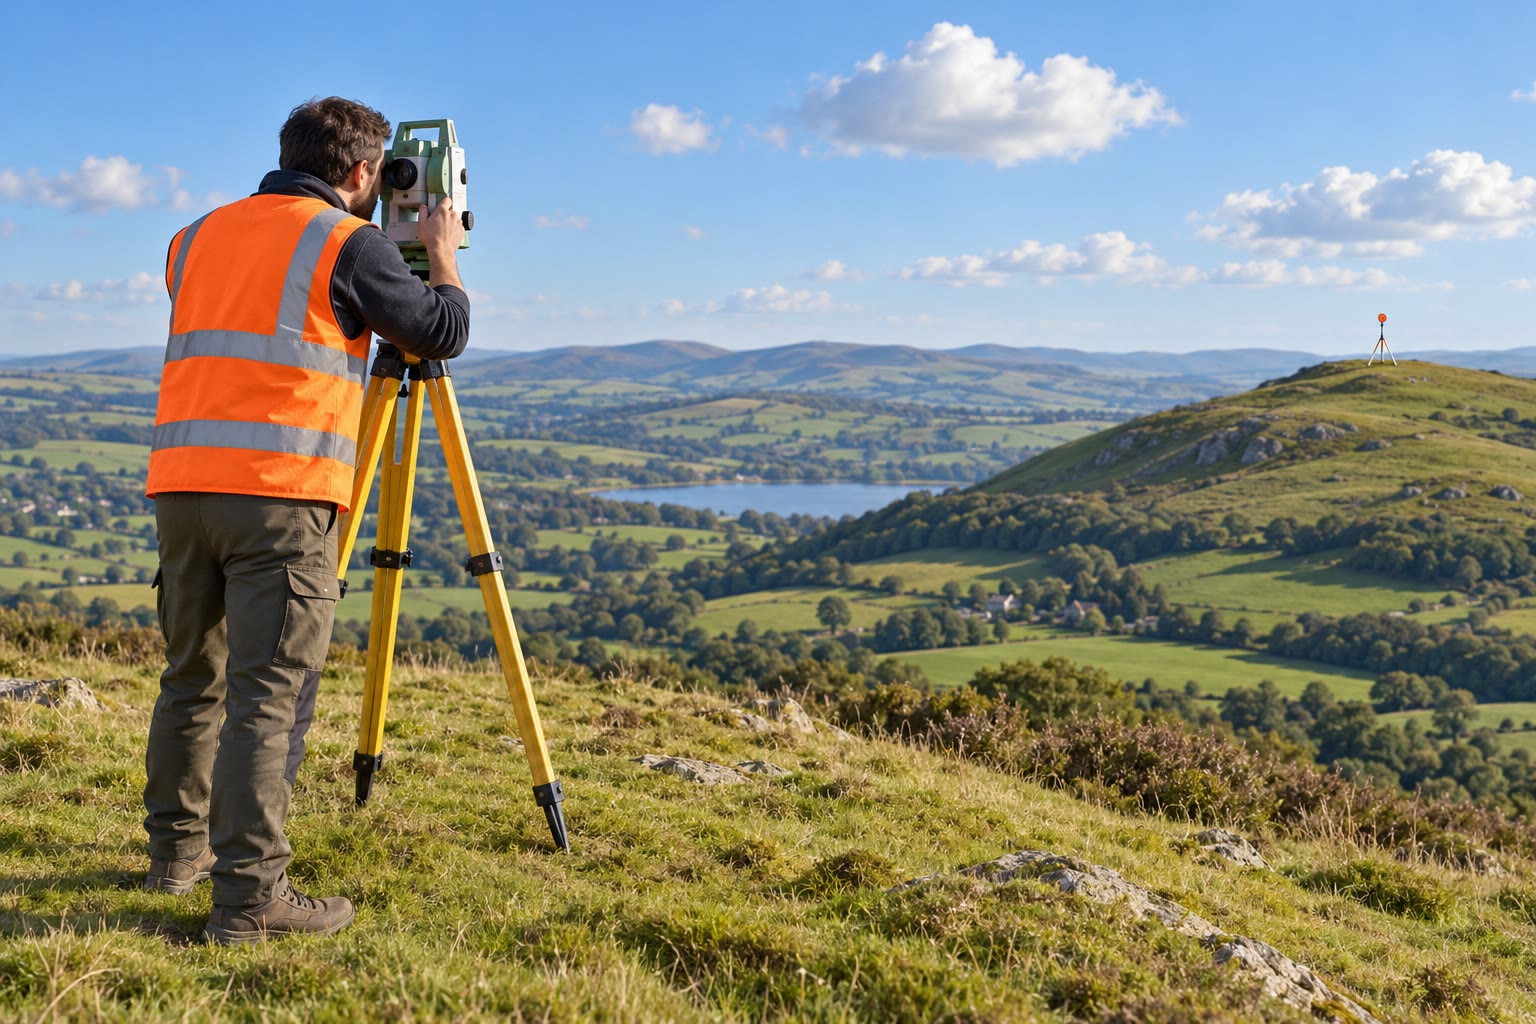
\includegraphics[width=0.7\linewidth]{images/book2/ai/g10-surveyor-theodolite.jpg}

{\small A surveyor at work with a modern instrument that measures angles
and, with a beam of light, distances; a survey signal stands on the far
hill.}
\end{omfigure}

The great \omterm{def:g10:measuring-the-earth:triangulation}{triangulations} of the eighteenth and nineteenth centuries have
been replaced by satellites. A receiver on the ground picks up the signals
of several satellites whose positions are known at every instant, and
computes its own position from the travel times of the signals (Book 1).
Networks of permanent receivers, fixed to bedrock all over the world,
measure their positions continuously. They define the reference frame in
which every map and every satellite position is given, and they move: they
show the plates of the lithosphere drifting by a few centimetres a year
(\cref{ch:g11:plate-motions}).
% ledger: usgs:gps

\begin{inthefield}[Measuring the ground today]
Geodesists anchor antennas on concrete pillars set in bedrock, far from
buildings and trees, and record their positions every few seconds for years.
They combine these with measurements from radio telescopes that observe very
distant galaxies and with laser beams fired at satellites carrying mirrors.
Surveyors on building sites and in the countryside still measure angles and
distances with instruments on tripods, and tie them to the satellite frame.
\end{inthefield}

\section{Exercises}

\begin{exercise}[$\star$]\label{exo:g10:measuring-the-earth:1}
Give three observations, possible without leaving the ground, that show
that the Earth is round. For each, explain in one sentence why a flat Earth
could not produce it.
\end{exercise}

\begin{exercise}[$\star$]\label{exo:g10:measuring-the-earth:2}
What is \omterm{def:g10:measuring-the-earth:geodesy}{geodesy}? What is \omterm{def:g10:measuring-the-earth:triangulation}{triangulation}, and which single length must be
measured on the ground in a \omterm{def:g10:measuring-the-earth:triangulation}{triangulation}?
\end{exercise}

\begin{exercise}[$\star$]\label{exo:g10:measuring-the-earth:3}
Eratosthenes found that the angle between the Sun's rays and the vertical at
Alexandria was $1/50$ of a full circle when the Sun was overhead at Syene,
5000 stadia away. Compute the circumference in stadia, then in kilometres,
taking a stadion of \qty{157.2}{m}.
\end{exercise}

\begin{exercise}[$\star$]\label{exo:g10:measuring-the-earth:4}
One degree of latitude is about \qty{111}{km} long. How long is one minute
of latitude ($1/60$ of a degree)? How long is the meridian from the equator
to the pole, roughly?
\end{exercise}

\begin{exercise}[$\star$]\label{exo:g10:measuring-the-earth:5}
Using the equatorial radius \qty{6378.137}{km} and the polar radius
\qty{6356.752}{km}, compute the difference of the two radii and the
\omterm{def:g10:measuring-the-earth:ellipsoid}{flattening} $f = (a-b)/a$. Express $f$ as one divided by a whole number.
\end{exercise}

\begin{exercise}[$\star\star$]\label{exo:g10:measuring-the-earth:6}
Two towns lie on the same meridian, \qty{500}{km} apart. At noon on the same
day, a vertical stick \qty{1.00}{m} high casts a shadow of \qty{0.364}{m} in
the southern town and of \qty{0.456}{m} in the northern town. Compute the
angle between the Sun's rays and the vertical in each town, then the
circumference of the Earth.
\end{exercise}

\begin{exercise}[$\star\star$]\label{exo:g10:measuring-the-earth:7}
In a triangle $ABC$, the baseline $AB = \qty{10.00}{km}$, the angle at $A$ is
\qty{62}{\degree} and the angle at $B$ is \qty{71}{\degree}. Compute the
angle at $C$ and the lengths $AC$ and $BC$.
\end{exercise}

\begin{exercise}[$\star\star$]\label{exo:g10:measuring-the-earth:8}
An aircraft flies due west along the parallel \qty{60}{\degree} N, from
longitude \qty{10}{\degree} E to longitude \qty{20}{\degree} W. Using a degree
of longitude of $111.3 \cos \varphi$ km, compute the distance it covers.
How long would the same change of longitude be on the equator?
\end{exercise}

\begin{exercise}[$\star\star$]\label{exo:g10:measuring-the-earth:9}
An observer's eye is $h = \qty{2}{m}$ above a calm sea. The line of sight to
the horizon grazes the sea at $T$; the centre of the Earth is $O$, the eye
$E$. Explain why the triangle $OTE$ has a right angle at $T$, then use
Pythagoras' theorem with $R = \qty{6371}{km}$ to show that the distance to
the horizon is about $\sqrt{2Rh}$, and compute it.
\end{exercise}

\begin{exercise}[$\star\star$]\label{exo:g10:measuring-the-earth:10}
Read the curve of degree lengths. Between which latitudes does the length of
a degree change fastest? Explain in two sentences why a degree of latitude is
longer near the poles than near the equator.
\end{exercise}

\begin{exercise}[$\star\star$]\label{exo:g10:measuring-the-earth:11}
The meridian arc from Dunkirk to Barcelona spans \qty{9.646}{\degree} of
latitude and is \qty{1072.2}{km} long. Compute the mean length of a degree
along it. If every degree had that length, how long would the quarter
meridian be? Compare with \qty{10002.0}{km} and explain the small
difference.
\end{exercise}

\begin{exercise}[$\star\star\star$]\label{exo:g10:measuring-the-earth:12}
Eratosthenes measured an angle of \qty{7.2}{\degree} and a distance of 5000
stadia. If his angle had been wrong by \qty{0.1}{\degree} (too small), by what
percentage would his circumference have been wrong, and in which direction?
Which of his two measurements do you think was the less precise?
\end{exercise}

\begin{exercise}[$\star\star\star$]\label{exo:g10:measuring-the-earth:13}
A chain of two triangles: in $ABC$, $AB = \qty{6.000}{km}$,
$A = \qty{55}{\degree}$, $B = \qty{75}{\degree}$. In the next triangle $ACD$,
built on the side $AC$, the angle at $A$ is \qty{50}{\degree} and the angle
at $C$ is \qty{68}{\degree}. Compute $AC$, then $AD$.
\end{exercise}

\begin{exercise}[$\star\star\star$]\label{exo:g10:measuring-the-earth:14}
At what latitude is a degree of longitude half as long as on the equator?
At what latitude is it one tenth as long? Explain why both answers do not
depend on the size of the Earth.
\end{exercise}

\begin{exercise}[$\star\star\star$]\label{exo:g10:measuring-the-earth:15}
Use the ellipsoid's values: a degree of latitude is \qty{110.574}{km} at the
equator and \qty{111.694}{km} at the pole. On a sphere of the same mean
radius, a degree would be \qty{111.195}{km} everywhere. By how many metres
would a surveyor who assumed a sphere be wrong over one degree at the
equator, and over one degree at the pole? Why must a map that gives
positions to the metre be computed on the ellipsoid?
\end{exercise}

\section{Problem: The Metre and the Meridian}

\begin{problem}[{Weekend problem --- from Eratosthenes' shadow to the length
of the first metre}]
\label{pb:g10:measuring-the-earth:1}
% ledger: geonames:aswan, geonames:alexandria, erat:method, metre:1791, metre:survey, wgs84:ellipsoid (arc lengths and degree lengths computed in figdata/grade-10/meridian_degree.py)
A student retraces the history of the measurement of the Earth with modern
numbers. Aswan, the ancient Syene, lies at latitude
\qty{24.09}{\degree} N and Alexandria at \qty{31.20}{\degree} N; on the
modern ellipsoid, the meridian arc between their two parallels is
\qty{788}{km} long. On the ellipsoid, one degree of latitude measures
\qty{110.57}{km} at the equator, \qty{111.13}{km} at \qty{45}{\degree} and
\qty{111.51}{km} at \qty{66}{\degree}, and the quarter meridian is
\qty{10001.966}{km}.

\medskip
\noindent\textbf{Part I --- Eratosthenes again.}
\begin{enumerate}
  \item Compute the difference of latitude between Aswan and Alexandria.
  \item What fraction of a full circle is it? Compare with Eratosthenes'
        $1/50$.
  \item Compute the circumference of the Earth that Eratosthenes' method
        gives with these modern numbers.
  \item The two cities are not on the same meridian: Aswan lies about
        \qty{3}{\degree} of longitude east of Alexandria. Which distance must
        be used in the method: the straight distance between the cities or
        the meridian arc between their parallels? Why?
  \item Why must the two shadows be measured on the same day, at local noon?
\end{enumerate}

\medskip
\noindent\textbf{Part II --- A small triangulation.}
A baseline $AB = \qty{12.000}{km}$ is measured. From $A$, the signal $C$ is
seen at \qty{58}{\degree} from $B$; from $B$, at \qty{66}{\degree} from $A$.
In the next triangle $ACD$, the angle at $A$ is \qty{47}{\degree} and the
angle at $C$ is \qty{75}{\degree}. The side $AD$ points \qty{8}{\degree}
east of north.
\begin{enumerate}[resume]
  \item Compute the angle at $C$ in the triangle $ABC$.
  \item Compute the side $AC$.
  \item Compute the side $BC$.
  \item Compute the angle at $D$ in the triangle $ACD$, then the side $AD$.
  \item Compute the north--south distance between $A$ and $D$.
  \item Using the degree length at \qty{45}{\degree}, compute the
        difference of latitude between $A$ and $D$, in degrees and in
        minutes of arc.
\end{enumerate}

\medskip
\noindent\textbf{Part III --- A flattened Earth.}
\begin{enumerate}[resume]
  \item By how many metres is a degree of latitude at \qty{66}{\degree}
        longer than one at the equator?
  \item Explain what this difference shows about the shape of the Earth.
  \item On the ellipsoid, $a = \qty{6378.137}{km}$ and
        $b = \qty{6356.752}{km}$. Compute $a - b$ and the \omterm{def:g10:measuring-the-earth:ellipsoid}{flattening}.
  \item Explain why, on a flattened Earth, the plumb line at a place of
        latitude \qty{45}{\degree} does not point exactly at the centre of
        the Earth.
\end{enumerate}

\medskip
\noindent\textbf{Part IV --- The first metre.}
\begin{enumerate}[resume]
  \item According to the definition of 1791, how long should the quarter
        meridian be, in metres?
  \item The platinum metre of 1799 was made from a measured value of the
        meridian. If the quarter meridian is in fact \qty{10001.966}{km},
        how long is one ten-millionth of it?
  \item Was the metre of 1799 too long or too short compared with its own
        definition? By what fraction?
  \item The platinum bar copied faithfully the length computed in the 1790s.
        Was the quarter meridian computed then too long or too short?
        Explain.
  \item By how many millimetres was the first metre shorter than one
        ten-millionth of the true quarter meridian? Compare with the
        thickness of a sheet of paper, about \qty{0.1}{mm}.
\end{enumerate}
\end{problem}
